\documentclass[number=1]{examfancy}

\newif\ifanswers
\answerstrue % comment out to hide answers
\ifanswers
 \def\answerspace{0}
  \def\longanswerspace{0}
\else
  \noprintanswers
%  \unframedsolutions
  \def\answerspace{60}
  \def\longanswerspace{100}
\fi

\begin{document}

\section*{Computer Architecture - \examtitle}

% Create header box, name and grade table
\makeboxheader
\makenameline
\makegradetable
\newpage

% Acronyms
\section*{List of commonly used acronyms}.
\begin{table}[!htb]
  \begin{tabular}{ll}
	\acrotable{CISC}\\
    \acrotable{IC}  \\
	\acrotable{ISA} \\
	\acrotable{RAM} \\
	\acrotable{RISC}\\
	\acrotable{uA}  \\
	\acrotable{uP}  \\
  \end{tabular}
\end{table}
\newpage

% Begin exam questions
\section*{Questions}.
\begin{questions}
% ========================================
\question[2] How many bits would you require in order to address a 4096-address \acs{RAM}?
\answer{\answerspace}{$\ceil{\log_{2}(4096)} = 12$}

% ========================================
\question[5] Define \acs{ISA}.
\answer{\longanswerspace}{\acs{ISA} is the link between an application and the physical layer of the computer.} 

% ========================================
\question[4] Describe the relation between \acs{uA} and \acs{ISA}.
\answer{\longanswerspace}{\acs{uA} defines how the \acs{ISA} is physically implemented.}

% ========================================
\question[4] What is throughput?
\answer{\longanswerspace}{The amount of tasks that we can perform in a given time. More specifically, it is the amount of bits we can output (process) in a given time. It is measured in bits/second.}

% ========================================
\question[4] What is latency?
\answer{\longanswerspace}{The amount of time taken for completing a task. It is measured in seconds.}

\newpage
% ========================================
\question[4] In the context of digital \acs{IC} design, what is synthesis?
\answer{\longanswerspace}{Synthesis is the process of generating logic gates from a \acs{HDL}.} 

% ========================================
\question[5] Define abstraction.
\answer{\longanswerspace}{Different representations of the same concept in order to deal with different levels of complexity that suits each designer's needs.} 

% ========================================
\question[2] One \acs{ISA} may be implemented using different \acsp{uA}.
\begin{choices}
\CorrectChoice True.
\choice False.
\end{choices}

% ========================================
\question[4] These are some \acs{ISA} characteristics.
\begin{choices}
\CorrectChoice Type and size of instructions and operands, instruction encoding, addressing modes, register types.
\choice Instruction encoding, type and size of memory, \acs{uA} implementation, power consumption.
\choice Addressing modes, instruction encoding, \acs{uA} implementation, latency.
\choice \acs{uA} implementation, addressing modes, type and size of instructions and operands, instruction encoding,  latency.
\end{choices}
\ifanswers
\else
\newpage
\fi
% ========================================
\question[3] Which of the following statements is correct.
\begin{choices}
\CorrectChoice Instruction encoding influences the \acs{uA} of an \acs{ISA}.
\choice \acs{uA} influences the instruction encoding of an \acs{ISA}.
\choice \acs{uA} and \acs{ISA} are not related.
\end{choices}

% ========================================
\question[3] Which types of memory addressing might be used in iterative constructs such as \code{for} loops?
\answer{\answerspace}{Autoincrement and autodecrement.}

\ifanswers
\newpage
\fi
% ========================================
\question[2] A single instruction encoding may be implemented using different \acsp{uA}.
\begin{choices}
\choice False.
\CorrectChoice True.
\end{choices}

% ========================================
\question[5] By a thorough inspection to an \acs{ISA}, we may be able to extract the following characteristics of a \acs{uP}.
\begin{choices}
\choice Whether the \acs{uP} is a \acs{CISC} or a \acs{RISC}, chip area, number of registers, types of memory addressing.
\choice Types of memory addressing, average number of clock cycles per instruction, size of main memory, power consumption.
\CorrectChoice Efficiency of memory usage of compiled programs, types of addressing modes.
\end{choices}

% ========================================
\question[5] Define instruction encoding.
\answer{\longanswerspace}{A convention, represented by binary codes, used to distinguish between the different instructions, operands and addressing modes of an \acs{ISA}.}

% ========================================
\question[4] What is the main difference between Harvard and Von-Neumann \acsp{uA}?
\answer{\longanswerspace}{A Harvard \acs{uA} uses separate buses for data and instructions, whilst a Von-Neumann \acs{uA} uses a single bus for both data and instruction.}

\newpage
% ========================================
\question[5] A \acs{uP} designer has made the decision to increase the number of supported instructions from 32 to 36. What does this design decision imply?
\begin{choices}
\choice The instruction encoding must be modified.\label{choice:q_designimplications_correct1}
\choice The technology (size of the transistors) of the \acs{uP} must be modified.\label{choice:q_designimplications_incorrect1}
\choice The size of the instruction memory must be modified.\label{choice:q_designimplications_incorrect2}
\choice The \acs{uA} must be modified.\label{choice:q_designimplications_correct2}
\choice All of the above.\label{choice:q_designimplications_incorrect3}
\choice None of the above.\label{choice:q_designimplications_incorrect4}
\choice Options \ref{choice:q_designimplications_correct1}, \ref{choice:q_designimplications_incorrect2} and \ref{choice:q_designimplications_correct2}. \label{choice:q_designimplications_incorrect5}
\CorrectChoice Options \ref{choice:q_designimplications_correct1} and \ref{choice:q_designimplications_correct2}.
\choice Options \ref{choice:q_designimplications_correct2}, \ref{choice:q_designimplications_incorrect1} and \ref{choice:q_designimplications_incorrect2}.\label{choice:q_designimplications_incorrect6}
\end{choices}

\newpage
% ========================================
\question[10] Classify the following \acs{ISA} characteristics into their corresponding \acs{CISC} or \acs{RISC} column. 
\\
\textbf{HINT.} Some characteristics might not fit into either column.
\begin{choices}
\choice More power consumption.\label{choice:incorrect_3}
\choice Limited addressing modes.\label{choice:risc_1}
\choice Microcode approach.\label{choice:cisc_1}
\choice Fixed-length encoding.\label{choice:risc_2}
\choice Instruction decoding is easily performed.\label{choice:risc_3}
\choice Multiple cycles per instruction.\label{choice:cisc_2}
\choice Yields smaller chip areas.\label{choice:incorrect_2}
\choice Load-store approach.\label{choice:risc_4}
\choice Reduced instruction memory usage.\label{choice:cisc_3}
\choice Uses one memory for instruction and one memory for data.\label{choice:incorrect_1}
\choice Variable-length encoding.\label{choice:cisc_4}
\choice Large number of addressing modes.\label{choice:cisc_5}
\choice Faster \acsp{uP}.\label{choice:incorrect_4}
\choice Single-cycle instructions.\label{choice:risc_5}
\end{choices}
\ifanswers
\answer{0}{
\begin{center}
\begin{tabular}{|c|c|}
\hline
~~~~~\acs{CISC}~~~~~ & ~~~~~\acs{RISC}~~~~~\\
\hline\hline
\ref{choice:cisc_1} & \ref{choice:risc_1} \\\hline
\ref{choice:cisc_2} & \ref{choice:risc_2} \\\hline
\ref{choice:cisc_3} & \ref{choice:risc_3} \\\hline
\ref{choice:cisc_4} & \ref{choice:risc_4} \\\hline
\ref{choice:cisc_5} & \ref{choice:risc_5} \\\hline\hline
\end{tabular}
\end{center}
}
\else
\renewcommand{\arraystretch}{1.7}
\begin{table}[!htb]
\centering
  \begin{tabular}{|c|c|}
  	\hline
	~~~~~\acs{CISC}~~~~~ & ~~~~~\acs{RISC}~~~~~\\ \hline\hline
& \\ \hline
& \\ \hline
& \\ \hline
& \\ \hline
& \\ \hline
& \\ \hline
& \\ \hline
& \\ \hline
& \\ \hline
& \\ \hline
  \end{tabular}
\end{table}
\renewcommand{\arraystretch}{1.0}


\fi


\newpage
% ========================================
\question[4] Assume that the machine code in~\fref{figure:cisc_code_hex} is obtained after compiling a piece of assembly code. What may we infer from the code of~\fref{figure:cisc_code_hex}?
\begin{figure}[!ht]
\centering
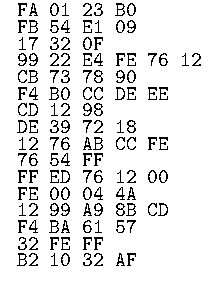
\includegraphics[scale=1.2]{cisc_code_hex}
\caption{Machine code in \code{HEX}.}
\label{figure:cisc_code_hex}
\end{figure}
\begin{choices}
\choice The size of the instruction memory.
\choice The number of clock cycles per instruction.
\choice The assembly code corresponds to a \acs{RISC}.
\choice All the above.
\CorrectChoice None of the above.
\end{choices}
\answer{0}{The code from~\fref{figure:cisc_code_hex} has variable-lenght encoding, which means that it corresponds to a \acs{CISC}.}

\newpage
% ========================================
\question[20] Assume that a \acs{uP} supports the instructions
\begin{center} 
\code{ADD}, \code{D}, \code{S1}, \code{S2} \\
\code{SUB}, \code{D}, \code{S1}, \code{S2}
\end{center}
for additions and subtractions, respectively.
The destination \code{D} could be either a \code{Reg} or a \code{Mem} location. 
Similarly, \code{S1} and \code{S2} correspond to the source of the operands and they may also be either a \code{Reg} or a \code{Mem} location.
Assume the notation of addressing modes shown in~\tref{table:addressing_modes}.

Using the registers and memory values shown in~\Cref{table:regs,table:mem}, respectively, complete \Cref{table:regs_fill,table:mem_fill} with the values of \code{Reg} and \code{Mem} after executing the operations shown in parts~\ref{part:address1} to~\ref{part:address4} of this question. 
Assume operations are independent from each other, \ie, the order of execution is not important and the result of one operation does not affect the execution of the rest.

\begin{table}[!h]
\centering
\caption{Memory addressing notation}
\label{table:addressing_modes}
\begin{tabular}{|c|c|}
\hline
Memory addressing & Notation \\
\hline\hline
Register          & \code{R}          \\\hline
Absolute          & \code{(constant)} \\\hline
Register indirect & \code{(R)}        \\\hline
Memory indirect   & \code{@(R)}       \\\hline
\end{tabular}
\end{table}
\begin{minipage}[b]{0.45\hsize}
\centering
\captionsetup{type=table}
\captionof{table}{\code{Reg} values}
\label{table:regs}
  \begin{tabular}{c|c}
  \code{Reg} & \code{Value} \\\hline
  \code{R1}  & \code{3} \\ 
  \code{R2}  & \code{11} \\ 
  \code{R3}  & \code{19} \\ 
  \code{R4}  & \code{31} \\ 
  \end{tabular}
\end{minipage}
\hfill
\begin{minipage}[b]{0.45\hsize}
\centering
\captionsetup{type=table}
\captionof{table}{\code{Mem} values}
\label{table:mem}
  \begin{tabular}{c|c}
  \code{Mem} & \code{Value} \\\hline
  \code{11}  & \code{5} \\ 
  \code{17}  & \code{41} \\ 
  \code{19}  & \code{43} \\ 
  \code{23}  & \code{29} \\ 
  \code{31}  & \code{11} \\ 
  \code{37}  & \code{13} \\ 
  \code{41}  & \code{23} \\ 
  \code{43}  & \code{53} \\ 
  \code{53}  & \code{59} \\ 
  \end{tabular}
\end{minipage}

\begin{parts}
\part \code{SUB}, \code{R1},   \code{(23)}, \code{R2}\label{part:address1}
\answer{0}{\code{R1} $\leftarrow$ \code{Mem[23] - R2} \\ 
\code{R1} $\leftarrow$ \code{29 - 11} \\ 
\code{R1} $\leftarrow$ \code{18} }
\part \code{ADD}, \code{(17)}, \code{(R2)},  \code{@(R4)}\label{part:address2}
\answer{0}{\code{Mem[17]} $\leftarrow$ \code{Mem[R2] + Mem[Mem[R4]]} \\
\code{Mem[17]} $\leftarrow$ \code{Mem[11] + Mem[Mem[31]]} \\
\code{Mem[17]} $\leftarrow$ \code{Mem[11] + Mem[11]} \\
\code{Mem[17]} $\leftarrow$ \code{5 + 5} \\
\code{Mem[17]} $\leftarrow$ \code{10}
}
\part \code{ADD}, \code{R2}, \code{(41)}, \code{R3}\label{part:address3}
\answer{0}{\code{R2} $\leftarrow$ \code{Mem[41] + R3} \\
\code{R2} $\leftarrow$ \code{23 + 19} \\
\code{R2} $\leftarrow$ \code{42} \\}
\part \code{SUB}, \code{@(R3)}, \code{(R4)}, \code{(11)}\label{part:address4}
\answer{0}{\code{Mem[Mem[R3]]} $\leftarrow$ \code{Mem[R4] - Mem[11]} \\
\code{Mem[Mem[19]]} $\leftarrow$ \code{Mem[31] - Mem[11]} \\
\code{Mem[43]} $\leftarrow$ \code{Mem[31] - Mem[11]} \\
\code{Mem[43]} $\leftarrow$ \code{11 - 5} \\
\code{Mem[43]} $\leftarrow$ \code{6} }

\renewcommand{\arraystretch}{2}
\begin{minipage}[b]{0.45\hsize}
\centering
\captionsetup{type=table}
\captionof{table}{\code{Reg} values}
\label{table:regs_fill}
  \begin{tabular}{c|c}
  \code{Reg} & Value \\
  \midrule
  \code{R1}  &  \\   \midrule
  \code{R2}  &  \\   \midrule
  \code{R3}  &  \\   \midrule
  \code{R4}  &  \\   \midrule
  \end{tabular}
\end{minipage}
\hfill
\begin{minipage}[b]{0.45\hsize}
\centering
\captionsetup{type=table}
\captionof{table}{\code{Mem} values}
\label{table:mem_fill}
  \begin{tabular}{c|c}
  \code{Mem} & Value \\
  \toprule
  \code{11}  &  \\   \midrule
  \code{17}  &  \\   \midrule
  \code{19}  &  \\   \midrule
  \code{23}  &  \\   \midrule
  \code{31}  &  \\   \midrule
  \code{37}  &  \\   \midrule
  \code{41}  &  \\   \midrule
  \code{43}  &  \\   \midrule
  \code{53}  &  \\   \midrule
  \end{tabular}
\end{minipage}
\renewcommand{\arraystretch}{1.0}

\end{parts}

\newpage
% ========================================
\question[5] What is a benchmark?
\answer{\longanswerspace}{A set of computer programs designed for measured the performance, for example latency, of a \acs{uP} or a complete computing system.}  
              
% ========================================
\question[5]\textbf{Bonus points question}. 

In which year did Pink Floyd release the album \emph{Dark side of the moon}?
\answer{\answerspace}{1973}  
                  
\end{questions}

\end{document}